\section{Introduction} \label{sec-introduction}

My research aims to find methods for modeling peripheral input when an embedded system firmware is rehosted or emulated. Rehosting involves executing firmware in an emulation environment instead of the original hardware. However, the emulation environments mainly do not include the peripherals hooked to the embedded system hardware. Modeling peripherals in rehosted embedded firmware helps keep the emulation environment close to the native hardware environment, thus higher fidelity. When testing, managing, or providing peripheral input, the input search space increases the code coverage and chances of discovering exploitable bugs. Peripheral input can be supplied from different paradigms, the emulation point of view, and the fuzzing lens. This area is an emerging field, especially from the fuzzing domain. Hence, I expanded the survey paper search space to include anything related to embedded system fuzzing and emulation.

Zhang et al.~\cite{zhang_firmware_2020} survey paper focused on using fuzz testing to find bugs in embedded system firmware. The paper reviewed twelve works and categorized them based on one criterion: the execution environment. Three of the twelve articles serve as platforms that allow plugins, and they neither fit the fuzzing firmware theme nor can find vulnerabilities. The paper does not provide enough relevant details on the topic, the type of firmware, fuzzing methods, etc. Also, the authors mentioned the targeted vulnerabilities but did not discuss them in detail. However, the pros and cons of reviewed works were partially addressed. The authors argue that simulation-based fuzz testing is the future but do not provide convincing arguments to back it up. The paper did suggest possible future work. The article has just four citations. I believe this is because it does not provide enough information about the state-of-the-art works and methods of the domain.


The authors of~\cite{wright_challenges_2022} addressed the problem of finding vulnerabilities in embedded systems from the system emulation perspective. The paper provides a comprehensive background on emulation, tools, and techniques. Also, the paper briefly discusses the vulnerability discovery techniques. Works are classified based on target system type, emulation approaches, emulation purpose, control, and fidelity. The authors further categorize challenges based on the emulation stage while discussing the process at each stage with diagrams in a detailed fashion. In addition, they compared methods and provided a guide on choosing the correct tool for system emulation and firmware rehosting, depending on the purpose. This paper has 44 citations, making it the highest-cited paper. I believe this is because it provides an organized view of the field and helps narrow down the challenges. Depending on the emulation stage, readers can find gaps in the area.


In~\cite{feng_detecting_2023}, the overarching theme is detecting vulnerabilities in IoT firmware. In addition to classifying IoT and embedded devices, the paper talks about techniques, their subcategories, and works that have adopted them. The authors also included figures and tables indicating the firmware security challenges the state-of-the-art works addressed and solutions. They further categorize challenges in emulation-based tests, albeit without a particular criterion. The paper suggested future directions. The paper included relevant information with a good structure. However, the paper took a top-down approach but did not buttress the core techniques.

Fasano et al.~\cite{fasano_sok_2021} paper is an example of a 70\% survey and 25\% research. The paper analyzes embedded system security in virtual or rehosted environments, hence from the emulation paradigm. The authors included figures of embedded system architectures depicting the used and unused peripherals. They also provide algorithms and scenarios that illustrate the need for dynamic analysis- testing at runtime. The paper then explains the challenges when building a virtual environment for firmware execution, such as fidelity evaluation, firmware acquisition, and peripheral modeling. In addition to the review, the article argues that it is impractical to emulate firmware with all peripherals modeled fully. The paper provides a roadmap to rehosting, discusses the state of the art, and suggests possible future direction. However, the work seems to assume readers have some prior knowledge and does not do a good job of bringing new researchers up to speed.

In a review on embedded systems fuzzing (ESF)~\cite{yun_fuzzing_2022}, issues of fuzzing on traditional software are compared and contrasted with those of embedded systems. The paper answers some research questions related to the ESF field. They are further classified based on the state-of-the-art fuzzing methods and algorithms that illustrate the fuzzing steps in detail. The authors also categorized based on the interfaces with which fuzzers interact with the firmware and the target application. The paper made suggestions for possible future work but does not argue based on limitations; rather, the suggestions were made from the trend in the domain.~\nocite{nadir_taxonomy_2022, qasem_automatic_2021, eisele_embedded_2022}



%\begin{figure}[ht!]
%\centerline{\includesvg[width=1.5\columnwidth]{images/mindmap.drawio.svg}}
%\caption{Example of using SVG on Overleaf}
%\label{fig: example}
%\end{figure}

\begin{figure}[ht]
    \begin{center}
        \centering
    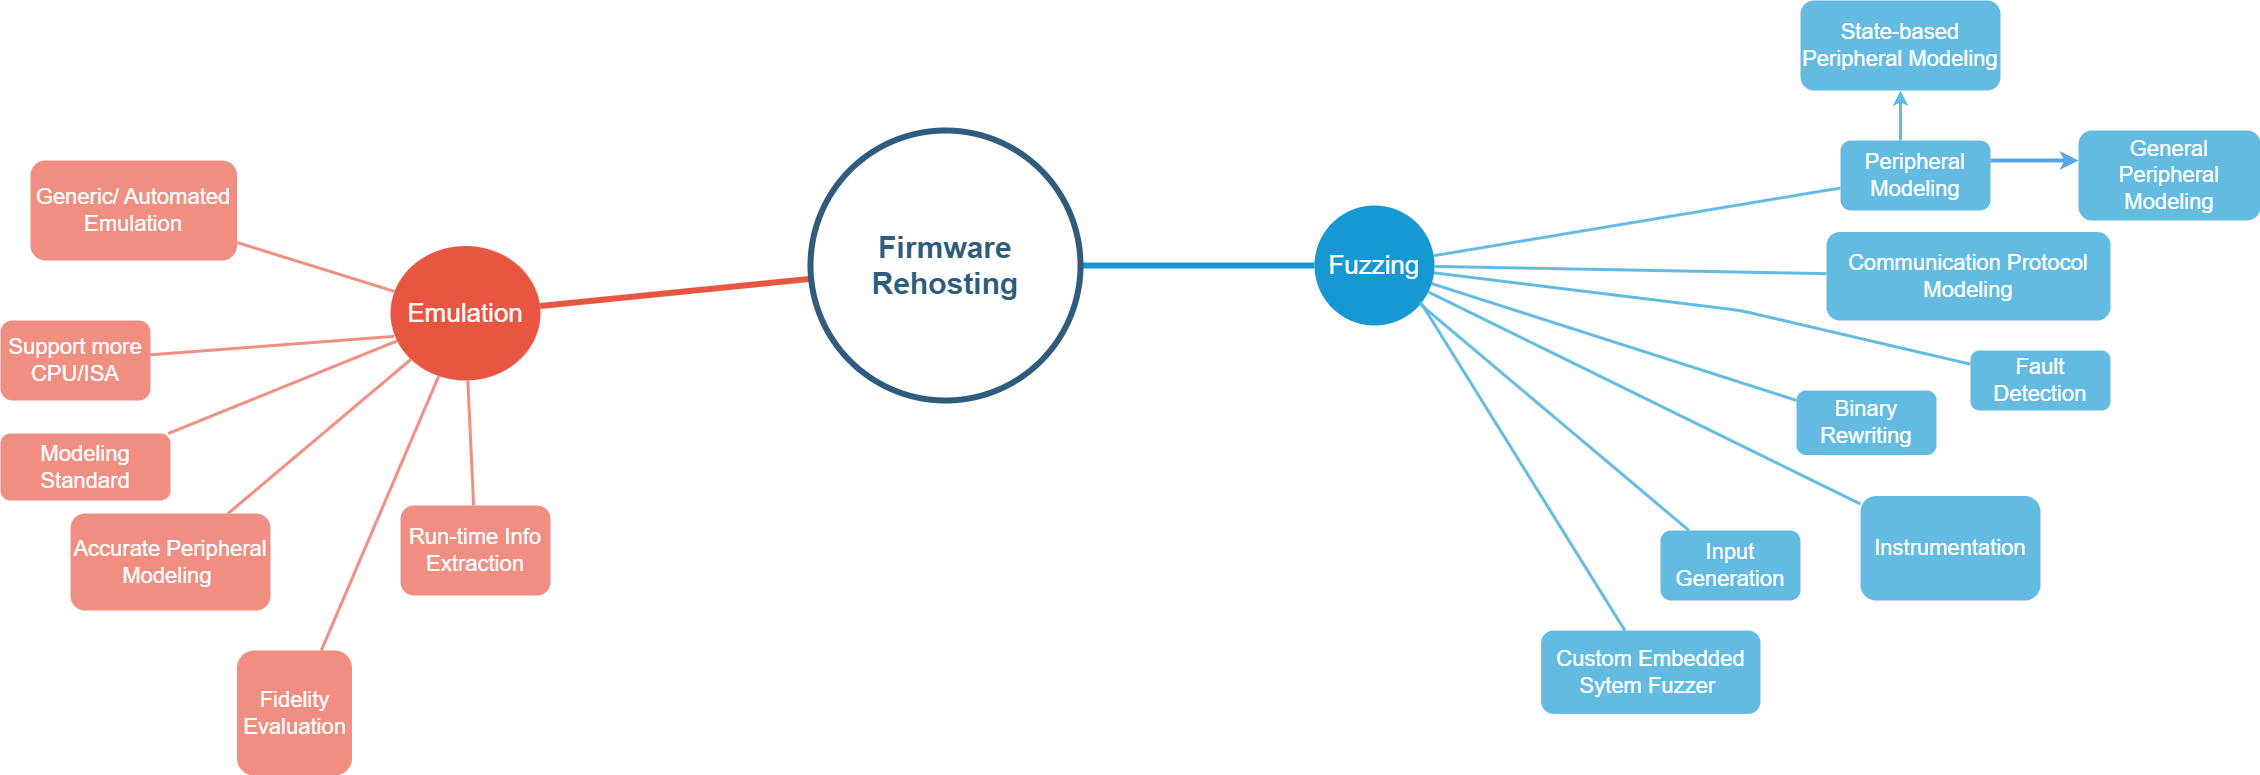
\includegraphics[width=6.5in]{images/mindmap.drawio.png}
    \caption{Mindmap showing gaps in the domain}
    \centering
    \label{fig:figure1}
    \end{center}    
\end{figure}